\documentclass[11pt,a4paper]{article}
\usepackage[margin=25mm]{geometry}
\usepackage{fontspec,unicode-math,booktabs,graphicx,array}
\setmainfont{STIXGeneral}\setmathfont{STIX Two Math}
\setlength{\parindent}{0pt}\setlength{\parskip}{5pt}
\begin{document}
\begin{center}{\Large Mix criteria: complete manuscript costs}\end{center}
The historical article is Cunningham and Hubard, \emph{Polytopality criteria
for the mix of polytopes and maniplexes}, arXiv:2506.19334v1, all 21 physical
pages. The comparison concerns its accepted corrected principal contract:
35 principal and background rows, with all three final problems still
unanswered. One original is compared with one complete application in two
papers, after paying for its entire common theory.

\textbf{Whole topic.} The primary ruler is literal untrimmed PDF extraction,
NFC characters without whitespace, fixed before counting. Titles, abstracts,
body, references, page footers and the source arXiv banner remain counted.
\begin{center}\begin{tabular}{lrr}\toprule
Complete document & Pages & Characters\\\midrule
Historical F005 source & 21 & 57753\\
Common theory $U$ & 5 & 12615\\
Local application $A_1$ & 8 & 20788\\
Exceptional application $A_2$ & 4 & 10289\\
Both complete code appendices & $4+3$ & 16025\\\bottomrule
\end{tabular}\end{center}
The written comparison charges both complete application papers:
\[
 R_{\mathrm{written}}=\frac{57753}{12615+20788+10289}
 =\frac{57753}{43692}=1.321821.
\]
After acquisition of the \emph{whole} common paper and \emph{all three}
complete mathematical programs, the one conditional comparison is
\[
 r\mid(U,P)=\frac{57753}{20788+10289}=\frac{57753}{31077}=1.858384.
\]
This conditional measure does not remove the acquisition from the whole-topic
cost. The exceptional correction receives no free prior-work allowance;
there is no overlap or cross-topic discount.

\textbf{Whole program alternatives.} One GAP file is a required finite
certificate for the coprime-label example. Two full Python files validate
written coordinate proofs. All three remain charged in these alternatives:
\[
 R_{\mathrm{printed}}=\frac{57753}{43692+16025}=0.967112,
 \qquad
 R_{\mathrm{raw}}=\frac{57753}{43692+14608}=0.990617.
\]
Printed and raw representations are alternatives, never simultaneous charges.
Both program-inclusive forms are longer than the source in this primary unit;
the sensitivity table preserves the different results in other units.
Three complete drivers cost 13674 characters separately; one full Lean
file costs 1714 separately and contains two generic declarations. Neither
is silently included in the displayed factors, and the full source is not
formalized. Historical software cost is unknown, rather than zero.

\newpage
\begin{center}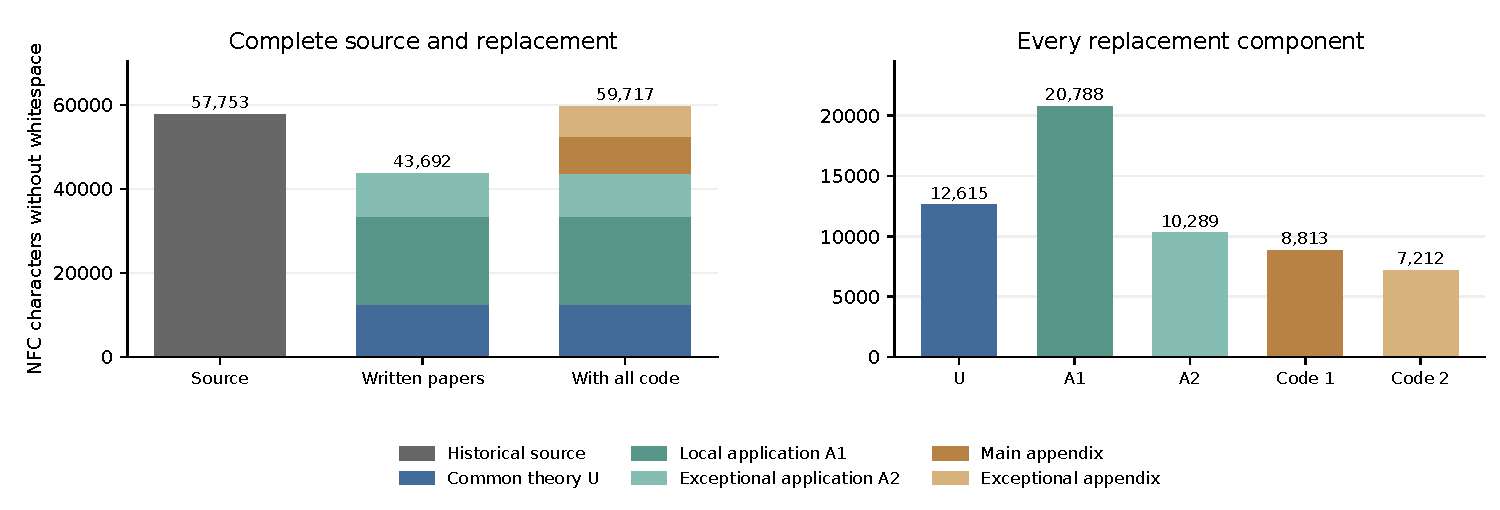
\includegraphics[width=\textwidth]{complete_costs.pdf}\end{center}
Both axes start at zero. The rectangles show the actual complete costs in the
primary unit, including both code appendices in the last total. The written
replacement is shorter by 14061 characters in this representation.
A single source supplies no recurring sawtooth pattern or theorem-node
compression statistic.

\textbf{Units and sensitivities.} For complete untrimmed text in NFC:
\begin{center}\small\begin{tabular}{lrrrr}\toprule
Unit & Written & Conditional & Printed & Raw code\\\midrule
Whitespace tokens & 1.442 & 2.026 & 1.232 & 1.258 \\
Alphanumeric units & 1.468 & 2.064 & 1.060 & 1.080 \\
Nonspace characters & 1.322 & 1.858 & 0.967 & 0.991 \\
Characters, spaces collapsed & 1.344 & 1.889 & 1.009 & 1.034 \\
UTF-8 bytes, spaces collapsed & 1.256 & 1.775 & 0.967 & 0.988 \\
\bottomrule\end{tabular}\end{center}
The JSON and CSV retain all five units under NFC and NFKC for untrimmed raw,
selected raw and calibrated selected text: thirty coordinates and 120 exact
fractions. The two selected sensitivities remove only isolated page footers;
nine visually checked glyph aliases affect only the calibrated sensitivity.
All source and replacement documents obey the same declared boundary.

\textbf{Scientific and measurement limits.} The accepted proofs include five
literal counterexample targets, including Corollaries 6.10(3) and 6.15(2),
and two further targets under the explicitly stated medial-component
convention. Their corrected rooted criteria and retained classical inputs
remain visible in the scientific source map. No answer to the three final
problems, new source credit or historical originality claim is made by this
measurement.

The accepted input audit binds 45 complete PDF pages, all three whole
mathematical programs, and the separate driver and formal inventories.
Extractable diagram labels and literal proxies are counted; full graphical
information, external proofs, software runtime, engineering and full
formalization costs remain unknown. These factors describe the declared text
representation, not minimum proof complexity or total research effort.
Distinct numerical review is required before publication.
\end{document}
